\documentclass[11pt,a4paper]{article}
\usepackage[T1]{fontenc}
\usepackage[utf8]{inputenc}
\usepackage[spanish,es-tabla,es-nodecimaldot,es-noshorthands]{babel}
\usepackage{lmodern}
\usepackage{microtype}
\usepackage[a4paper,top=2.4cm,bottom=2.4cm,left=2.3cm,right=2.3cm,headheight=15pt]{geometry}
\usepackage{amsmath,amssymb}
\usepackage[output-decimal-marker={,}]{siunitx}
\usepackage{booktabs,array,tabularx}
\usepackage{graphicx,float}
\usepackage[font=small,labelfont=bf,labelsep=period]{caption}
\usepackage[table]{xcolor}
\usepackage[most]{tcolorbox}
\usepackage{fancyhdr,lastpage}
\usepackage{enumitem}
\usepackage{titlesec}
\usepackage[hidelinks]{hyperref}
\definecolor{azul}{HTML}{1C5CAB}
\definecolor{gris}{HTML}{52514E}
\titleformat{\section}{\Large\bfseries\color{azul}}{\thesection}{0.8em}{}[\vspace{-0.6ex}\color{azul!40}\rule{\linewidth}{0.6pt}]
\titleformat{\subsection}{\large\bfseries\color{azul}}{\thesubsection}{0.8em}{}
\setlength{\parskip}{0.45em}\setlength{\parindent}{0pt}
\pagestyle{fancy}\fancyhf{}
\fancyhead[L]{\small\color{gris}Mitras KG m\,0,5 $\times$ 20 --- Torque admisible según Shigley}
\fancyhead[R]{\small\color{gris}Informe técnico}
\fancyfoot[C]{\small\color{gris}Página \thepage\ de \pageref{LastPage}}
\renewcommand{\headrulewidth}{0.4pt}
\newtcolorbox{caja}[2][azul]{colback=#1!5,colframe=#1,boxrule=0.6pt,arc=1mm,left=2mm,right=2mm,top=1mm,bottom=1mm,fonttitle=\bfseries,title={#2}}
\setlist{itemsep=0.2em,topsep=0.3em}
\graphicspath{{./}}
\begin{document}
\begin{titlepage}
\centering
\vspace*{2.2cm}
{\color{azul}\rule{\linewidth}{1.2pt}}\\[0.8cm]
{\Huge\bfseries Torque admisible de un par de\\[0.25cm] engranajes cónicos KG m\,0,5 $\times$ 20\\[0.25cm] para la transmisión a 90$^\circ$ de una rueda\par}
\vspace{0.6cm}
{\Large Análisis según Shigley (método AGMA para engranajes cónicos),\\ alternativas de mayor capacidad y lubricación\par}
\vspace{0.6cm}
{\color{azul}\rule{\linewidth}{1.2pt}}\\[1.4cm]
\begin{tabular}{rl}
\textbf{Producto analizado:} & KG STOCK GEARS, mitra serie M, $m=0{,}5$ mm, $z=20$\\
\textbf{Materiales:} & S45C, SUS304L (MIM), latón C3604B, POM inyectado\\
\textbf{Velocidades:} & 0, 0,5, 50 y 100 rpm\\
\textbf{Confiabilidad:} & 95\,\%\\
\textbf{Servicio:} & rueda de carro, torque en ambos sentidos, picos de 10 s\\
\textbf{Método:} & Budynas y Nisbett, \textit{Diseño en ingeniería mecánica de Shigley}, cap. 15\\
\end{tabular}
\vfill
{\large Informe técnico\\ Septiembre de 2026\par}
\end{titlepage}

\section*{Resumen ejecutivo}
\addcontentsline{toc}{section}{Resumen ejecutivo}
Se determinó el torque admisible del par de mitras KG m\,0,5 $\times$ 20 que transmite el giro a la rueda de un carro,
para cada material en que el fabricante ofrece la pieza. Se usaron las ecuaciones AGMA para engranajes cónicos
del capítulo~15 de Shigley. Como la rueda recibe torque en ambos sentidos, la resistencia a flexión se toma como alternada (70\,\%).
La confiabilidad es del 95\,\%. El servicio combina un torque normal bajo durante toda la vida con picos ocasionales de 10~s.

\begin{table}[H]\centering\small
\caption{Torque admisible por engranaje, en N\,m ($R=0{,}95$, carga en ambos sentidos, 10 años).}\label{tab:resumen}
\begin{tabular}{l ccc cccc}
\toprule
 & \multicolumn{3}{c}{Torque normal (toda la vida)} & \multicolumn{4}{c}{Torque de pico (10 s, ocasional)}\\
\cmidrule(lr){2-4}\cmidrule(lr){5-8}
Material & 0,5 rpm & 50 rpm & 100 rpm & 0 rpm & 0,5 rpm & 50 rpm & 100 rpm\\
\midrule
S45C & 0,129 & 0,083 & 0,076 & 0,195 & 0,194 & 0,147 & 0,133 \\
SUS304L (MIM) & 0,052 & 0,033 & 0,032 & 0,078 & 0,078 & 0,059 & 0,053 \\
Latón C3604B & 0,063 & 0,040 & 0,039 & 0,094 & 0,094 & 0,071 & 0,065 \\
POM inyectado$^{*}$ & 0,025 & 0,020 & 0,020 & 0,021 & 0,029 & 0,027 & 0,026 \\
\bottomrule
\end{tabular}

\smallskip\footnotesize $^{*}$POM: fuera del alcance de AGMA; método de Lewis (sección~\ref{sec:pom}).
\end{table}


\begin{caja}{Conclusiones principales}
\begin{enumerate}[leftmargin=1.2em]
\item \textbf{S45C es la mejor opción de KG}: admite 0,076~N\,m en servicio normal a 100~rpm,
0,133~N\,m en picos de 10~s a 100~rpm y 0,195~N\,m a rueda detenida.
\item El dato del catálogo KG (1,5~W a 100~rpm $=$ 0,143~N\,m) no sirve para este uso. Es solo a flexión, en un solo sentido,
y extrapola una norma que empieza en $m=1{,}5$. Supera en un 88\,\% la capacidad normal calculada.
\item \textbf{Dentro de $d_a\le14$ mm} hay margen. La mitra KG m\,0,5 $\times$ 25 de stock (alternativa B) casi duplica la capacidad
($\times$1,8). Una mitra a medida m\,0,6 $\times$ 21
carburizada la multiplica por 6,3 (sección~\ref{sec:alt}).
\item \textbf{La lubricación es imprescindible} en los metales: los valores AGMA presuponen engranajes lubricados.
A la velocidad de trabajo la película es de lubricación límite, así que se requiere grasa con aditivos EP (sección~\ref{sec:lub}).
\end{enumerate}
\end{caja}

\tableofcontents
\newpage

\section{Objeto y datos de partida}
\subsection{Aplicación}
El par de mitras transmite el giro de un motor BLDC a la rueda de un carro, con ejes a 90$^\circ$ y relación 1:1.
El compartimiento está engrasado y la temperatura de trabajo es de 30 a 40\,$^\circ$C. El motor sigue un perfil
trapezoidal suave. El equipo se usa 20~h seguidas una vez por mes.

\subsection{Ciclo de carga de la rueda}
\begin{itemize}
\item \textbf{Torque en ambos sentidos.} Marcha adelante y atrás, aceleración y frenado. Cada diente se flexiona hacia
uno y otro lado, así que Shigley indica usar el 70\,\% de la resistencia a flexión.
\item \textbf{Servicio normal} con torque bajo durante toda la vida: $N_{normal}=n\cdot60\cdot20\cdot12\cdot10$ ciclos por diente.
\item \textbf{Picos ocasionales} al torque admisible, de 10~s cada uno. Se supuso \textbf{un pico por hora de uso}:
$N_{picos}=2400$ eventos en 10 años. Cada pico suma $\max(1;\,n\cdot10/60)$ ciclos por diente.
\item \textbf{Combinación (regla de Miner).} A cada régimen se le asigna la mitad del daño admisible, así que su resistencia se evalúa al
doble de sus ciclos:
\begin{equation}
\frac{n_{normal}}{N_{normal}}+\frac{n_{pico}}{N_{pico}}=0{,}5+0{,}5=1
\quad\Rightarrow\quad N_{eval}=2\,n .
\end{equation}
\end{itemize}

\begin{table}[H]\centering\small
\caption{Datos, supuestos y su origen.}
\begin{tabularx}{\linewidth}{l X l}
\toprule
Dato & Valor & Origen\\\midrule
Par & Dos mitras iguales, 1:1, $\Sigma=90^\circ$ & pedido\\
Producto & KG serie M, $m=0{,}5$ mm, $z=20$, $b=2{,}5$ mm & catálogo KG\\
Velocidades & 0, 0,5, 50 y 100 rpm (el pedido admite leer <<0,50 rpm>>; se calcularon ambas) & pedido\\
Confiabilidad & $R=0{,}95$ & pedido\\
Uso & 20 h por mes; vida de diseño 10 años (2400 h) & pedido / \textbf{supuesto}\\
Picos & 10 s, 1 por hora de uso (2400 en la vida) & pedido / \textbf{supuesto}\\
Carga & BLDC, perfil trapezoidal suave, torque en ambos sentidos & pedido\\
Lubricación & Grasa en compartimiento cerrado & pedido\\
Temperatura & 30--40\,$^\circ$C (se calcula a 40\,$^\circ$C) & pedido\\
Montaje & Ambos engranajes en voladizo & \textbf{supuesto} conservador\\
\bottomrule
\end{tabularx}
\end{table}

\section{El producto KG y el alcance de su dato de capacidad}
\subsection{Materiales disponibles en m\,0,5 $\times$ 20}
El catálogo vigente de KG (KG4001) ofrece la mitra m\,0,5 de 20 dientes en S45C (M50S20), inoxidable SUS304L inyectado (MIM, M50SUM20)
y latón C3604B (M50B20). El POM azul y el blanco empiezan en m\,0,8. El catálogo 2020 (KG3001) incluía además
una versión de POM negro inyectado (M50DM20-1103).
\begin{figure}[H]\centering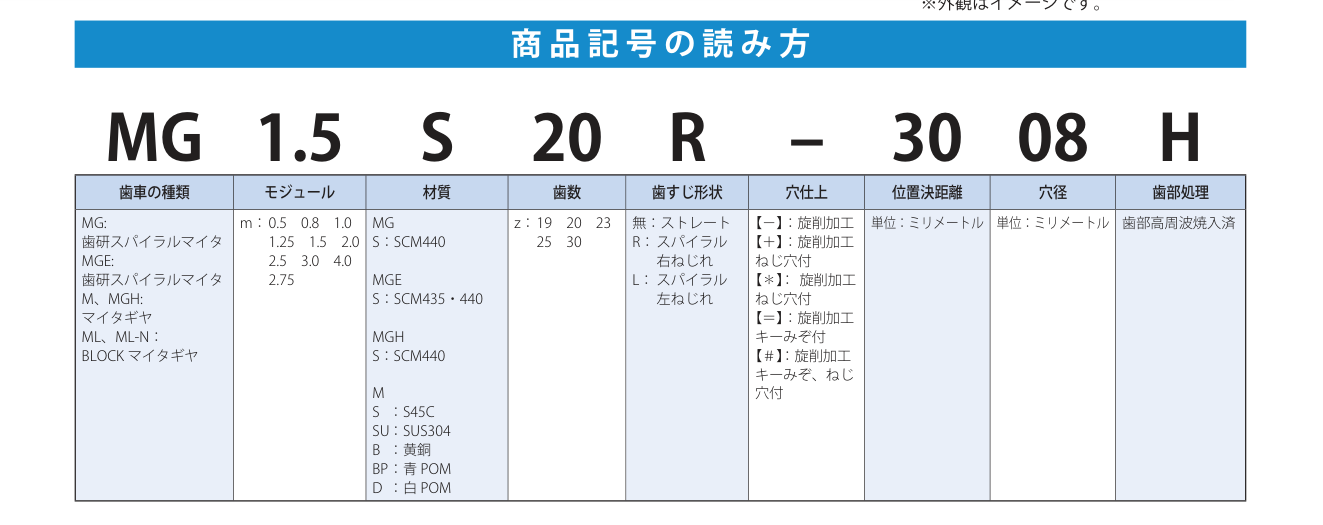
\includegraphics[width=0.95\linewidth]{capturas/kg_codigo_producto.png}\caption{Código de producto de las mitras KG. \textit{Fuente: KG, catálogo KG4001, p. 233.}}\end{figure}

\begin{figure}[H]\centering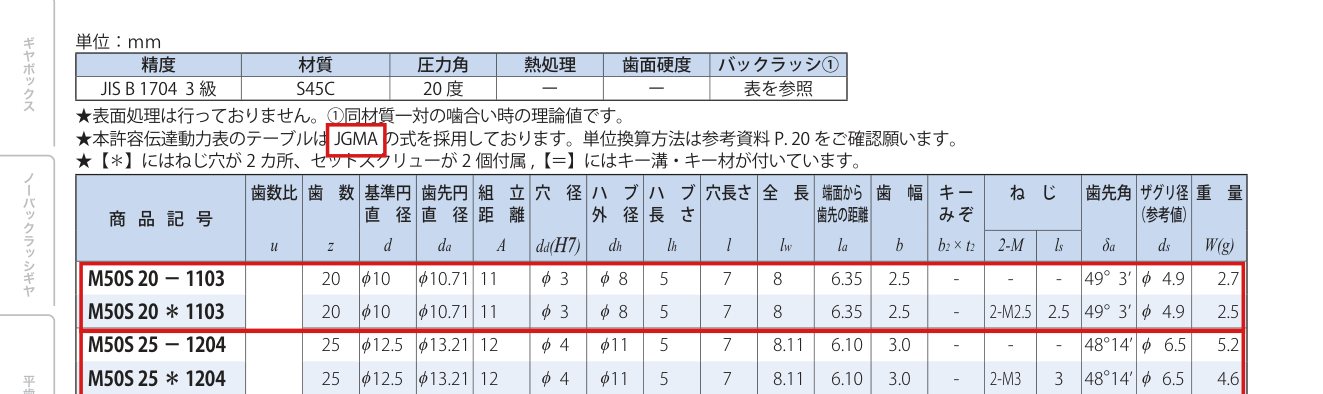
\includegraphics[width=\linewidth]{capturas/kg_s45c_datos.png}\caption{Mitra S45C m\,0,5 $\times$ 20 (M50S20): JIS B1704 grado 3, sin tratamiento térmico, $b=2{,}5$ mm, $d=10$ mm. \textit{Fuente: KG, catálogo KG4001, p. 260.}}\end{figure}

\begin{figure}[H]\centering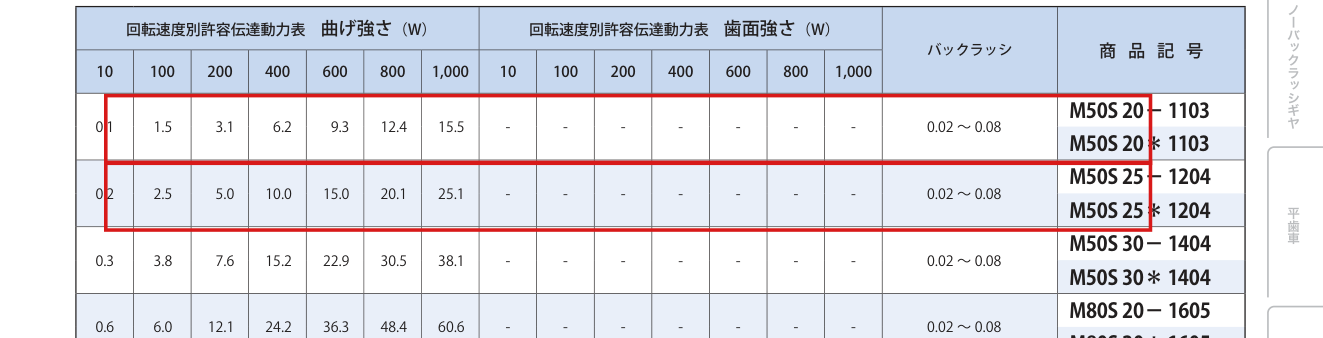
\includegraphics[width=\linewidth]{capturas/kg_s45c_potencia.png}\caption{Potencia admisible de M50S20: 1,5 W a 100 rpm a flexión; la resistencia superficial no se publica («--»). \textit{Fuente: KG, catálogo KG4001, p. 261.}}\end{figure}

\begin{figure}[H]\centering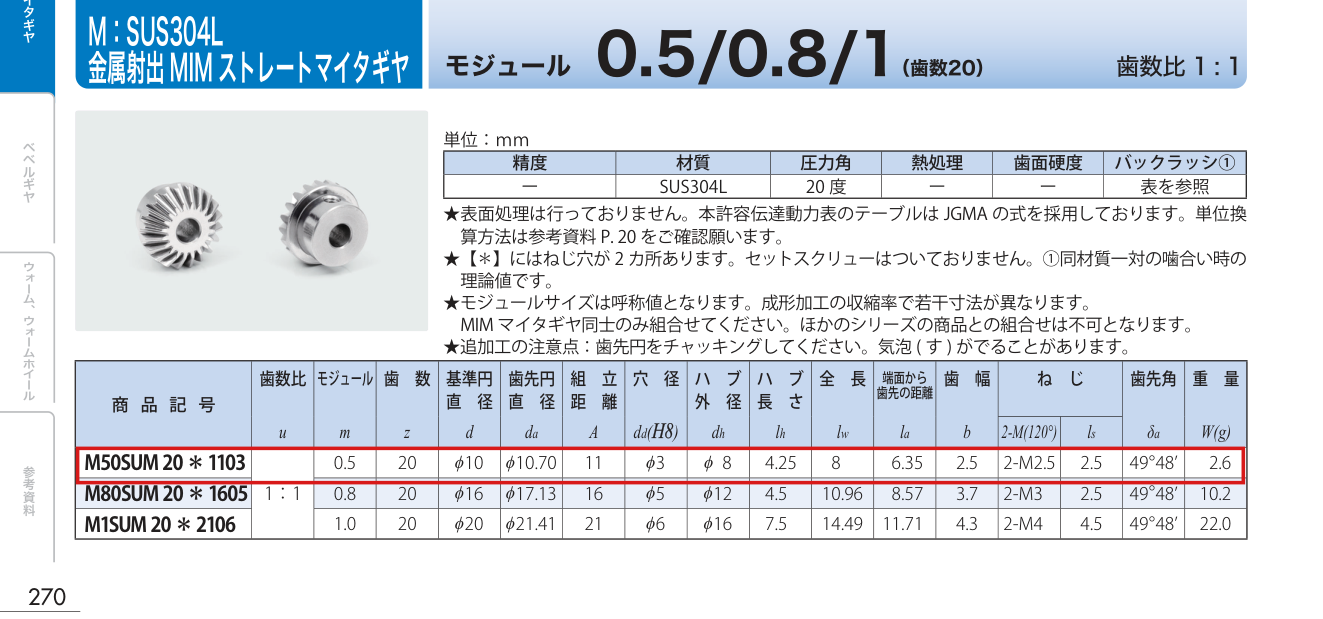
\includegraphics[width=0.9\linewidth]{capturas/kg_mim_datos.png}\caption{Mitra SUS304L MIM m\,0,5 $\times$ 20 (M50SUM20*1103): sin prisioneros y solo combinable con otra mitra MIM. \textit{Fuente: KG, catálogo KG4001, p. 270.}}\end{figure}

\begin{figure}[H]\centering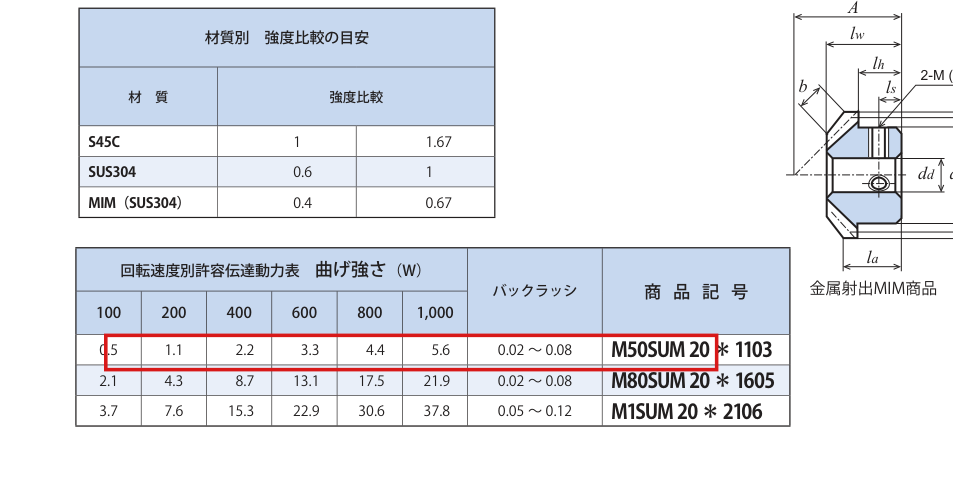
\includegraphics[width=0.8\linewidth]{capturas/kg_mim_potencia.png}\caption{Potencia admisible de M50SUM20 (0,5 W a 100 rpm) y relación orientativa de resistencia: S45C 1, SUS304 0,6, MIM 0,4. \textit{Fuente: KG, catálogo KG4001, p. 271.}}\end{figure}

\begin{figure}[H]\centering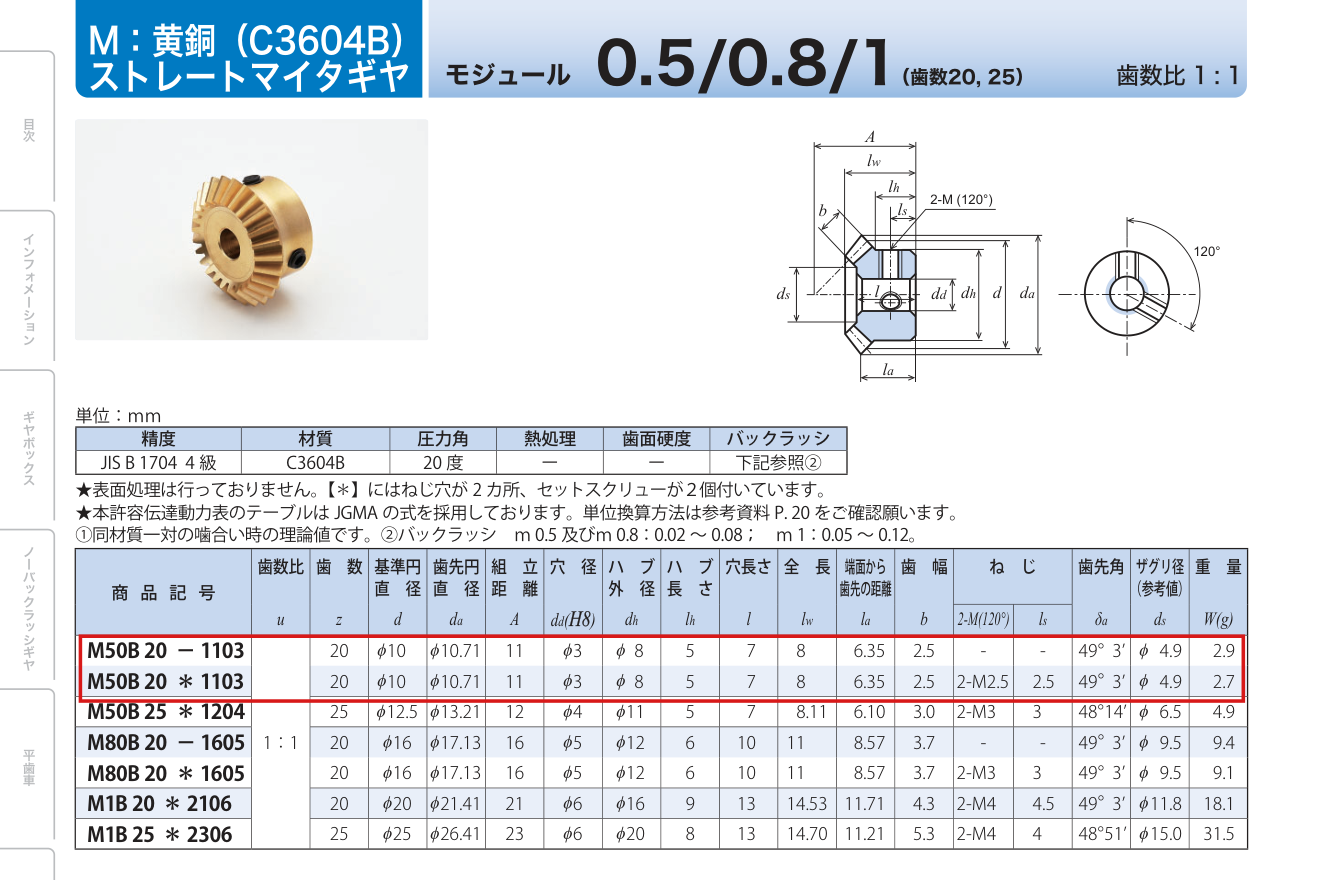
\includegraphics[width=0.9\linewidth]{capturas/kg_laton_datos.png}\caption{Mitra de latón C3604B m\,0,5 (M50B20 y M50B25); sin tabla de potencia. \textit{Fuente: KG, catálogo KG4001, p. 272.}}\end{figure}

\begin{figure}[H]\centering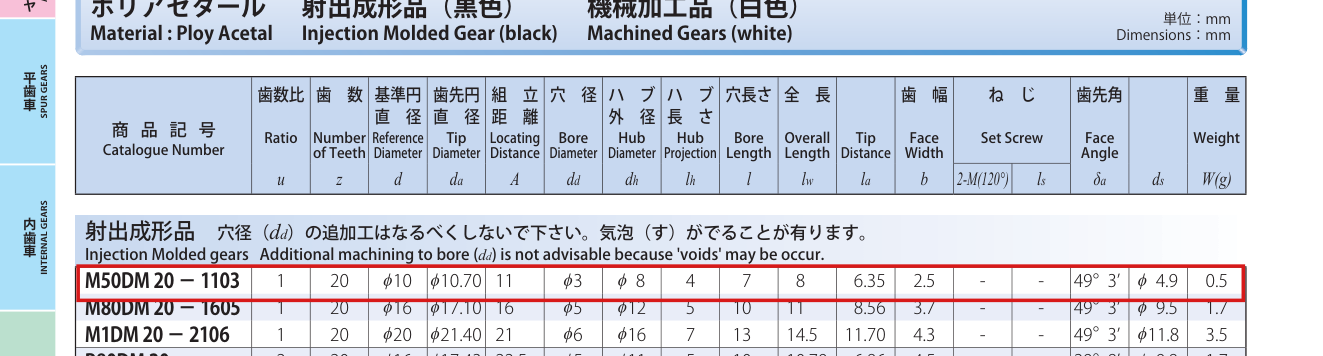
\includegraphics[width=\linewidth]{capturas/kg_pom_datos.png}\caption{Mitra de POM negro inyectado m\,0,5 $\times$ 20 (M50DM20-1103), catálogo 2020. \textit{Fuente: KG, catálogo KG3001, p. 400.}}\end{figure}


\subsection{Qué cubre el dato de KG}
\begin{figure}[H]\centering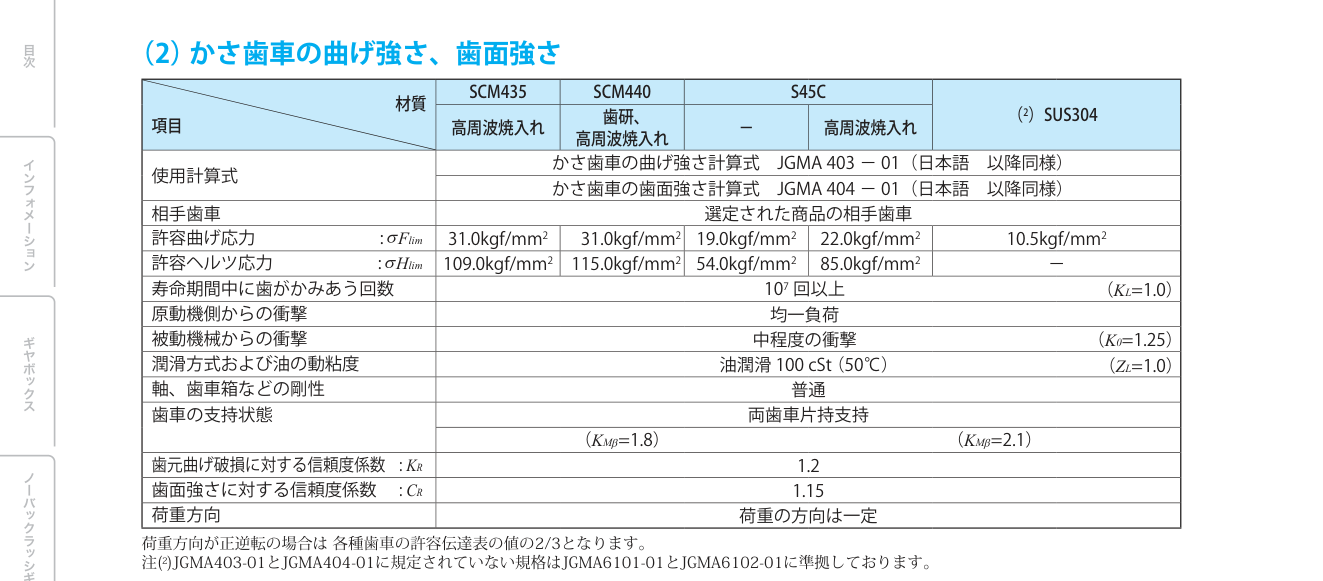
\includegraphics[width=\linewidth]{capturas/kg_condiciones_conicos.png}\caption{Condiciones de las tablas de KG para cónicos: JGMA 403-01/404-01; $\geq10^7$ ciclos; choque moderado ($K_O=1{,}25$); baño de aceite 100 cSt; ambos engranajes en voladizo; con carga en ambos sentidos, 2/3 del valor de tabla. \textit{Fuente: KG, KG5001, p. 18.}}\end{figure}

\begin{figure}[H]\centering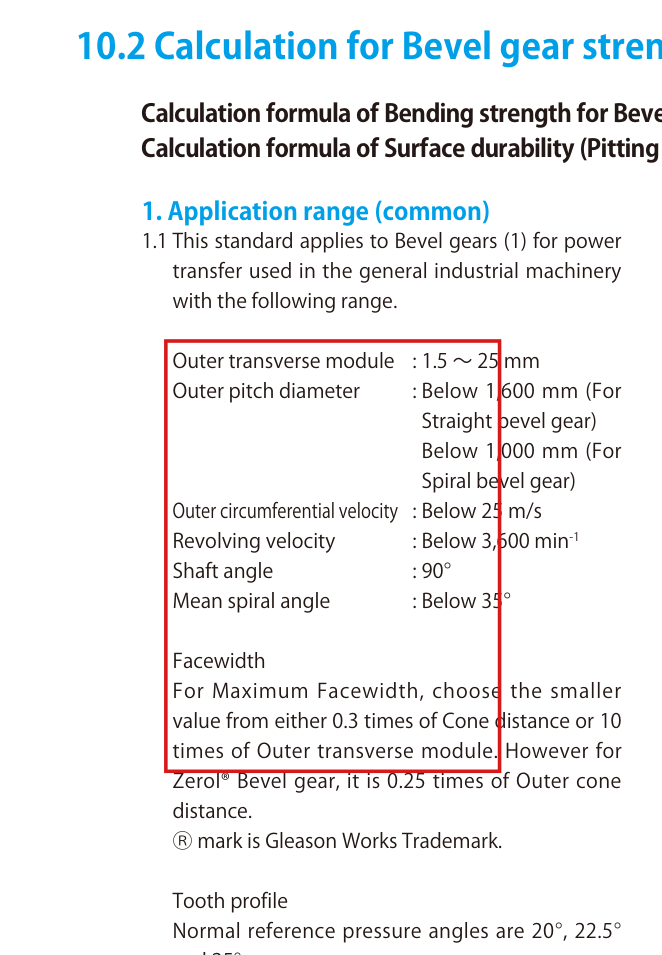
\includegraphics[width=0.48\linewidth]{capturas/kg_jgma403_alcance.png}\caption{Alcance de JGMA 403-01/404-01: módulo exterior de 1,5 a 25 mm. \textit{Fuente: KG, Technical Data, cap. 10.2, p. 137.}}\end{figure}

\begin{figure}[H]\centering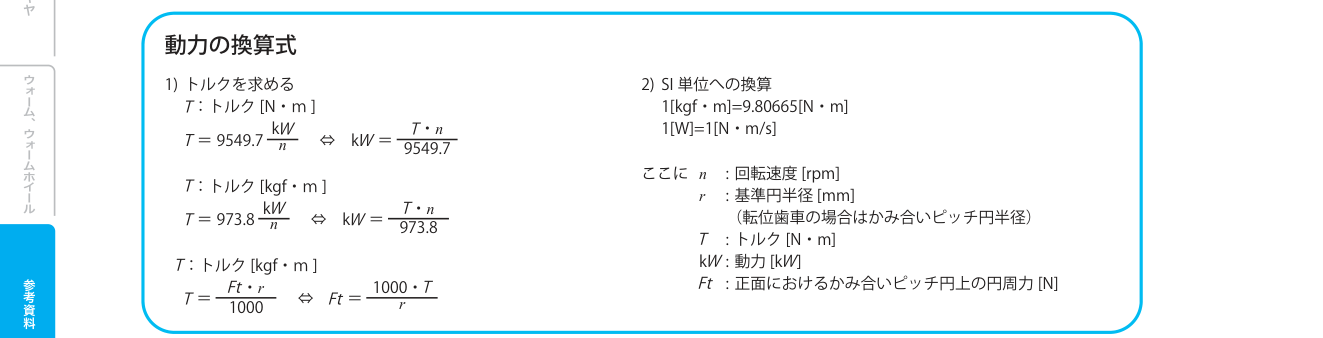
\includegraphics[width=\linewidth]{capturas/kg_conversion_potencia.png}\caption{Conversión de potencia a torque: $T\,[\mathrm{N\,m}]=9549{,}7\,P\,[\mathrm{kW}]/n$. \textit{Fuente: KG, KG5001, p. 20.}}\end{figure}


\begin{caja}[orange!80!black]{Limitaciones del dato del fabricante}
\begin{enumerate}[leftmargin=1.2em]
\item Solo publica flexión. Para m\,0,5 no hay resistencia superficial (picado).
\item Usa JGMA 403/404, cuyo alcance empieza en $m=1{,}5$ mm.
\item Supone carga en un sentido, baño de aceite y $\geq10^7$ ciclos, condiciones distintas a las de una rueda.
\item El latón y el POM m\,0,5 no tienen dato. El del MIM es experimental (catálogo 2020).
\end{enumerate}
\end{caja}

\section{Geometría}
\begin{minipage}[c]{0.46\linewidth}\centering
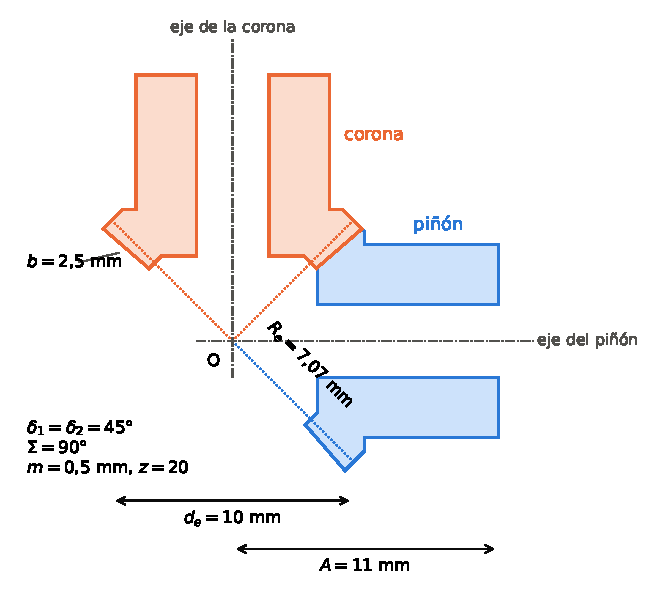
\includegraphics[width=\linewidth]{figuras/fig_geometria.pdf}
\captionof{figure}{Corte axial esquemático del par.}
\end{minipage}\hfill
\begin{minipage}[c]{0.5\linewidth}\small
\begin{tabular}{l r}
\toprule
Magnitud & Valor\\\midrule
Módulo exterior $m_{et}$ & 0,5 mm\\
Dientes $z_1=z_2$ & 20\\
Ángulo de presión $\phi$ & 20$^\circ$\\
Diámetro primitivo $d_e=m\,z$ & 10,0 mm\\
Ángulo de paso $\delta$ & 45$^\circ$\\
Distancia de cono $R_e=d_e/(2\sin\delta)$ & 7,071 mm\\
Ancho de catálogo $b$ & 2,5 mm\\
Máximo recomendado $0{,}3R_e$ & 2,121 mm\\
\textbf{Ancho efectivo} $b_{ef}$ & \textbf{2,121 mm}\\
Diámetro exterior $d_a$ & 10,71 mm\\
Dientes virtuales $z_v=z/\cos\delta$ & 28,28\\
$v_{et}$ a 100 rpm & 0,0524 m/s\\
\bottomrule
\end{tabular}
\end{minipage}

El ancho de catálogo supera el 30\,\% de la distancia de cono ($b/R_e=0,354$), límite que recomienda Shigley.
Por eso solo se acredita $b_{ef}=0{,}3R_e$.

\section{Método de cálculo (Shigley, capítulo 15)}
Shigley presenta las ecuaciones de ANSI/AGMA 2003 para engranajes cónicos rectos. En unidades SI, con $W^t$ la fuerza
tangencial en el diámetro primitivo exterior:

\paragraph{Esfuerzo de contacto (picado).}
\begin{equation}
\sigma_H = Z_E\left(\frac{W^t}{b\,d_{e1}\,Z_I}\,K_A K_v K_{H\beta} Z_x Z_{xc}\right)^{1/2}
\le \sigma_{HP}=\frac{\sigma_{H\,\lim}\,Z_{NT}\,Z_W}{S_H\,K_\theta\,Z_Z}
\label{eq:contacto}
\end{equation}

\paragraph{Esfuerzo de flexión.}
\begin{equation}
\sigma_F = \frac{W^t}{b}\,\frac{K_A K_v}{m_{et}}\,\frac{Y_x K_{H\beta}}{Y_\beta\,Y_J}
\le \sigma_{FP}=\frac{0{,}70\,\sigma_{F\,\lim}\,Y_{NT}}{S_F\,K_\theta\,Y_Z}
\label{eq:flexion}
\end{equation}
El factor $0{,}70$ corresponde a la carga en ambos sentidos.

\paragraph{Torque admisible.} Se despeja $W^t$ de \eqref{eq:contacto} y \eqref{eq:flexion}, con $T=W^t d_e/2$:
\begin{align}
T_F &= \frac{d_e}{2}\;\frac{\sigma_{FP}\;b\;m_{et}\;Y_\beta\,Y_J}{K_A\,K_v\,Y_x\,K_{H\beta}}\\[4pt]
T_H &= \frac{d_e}{2}\left(\frac{\sigma_{HP}}{Z_E}\right)^{2}\frac{b\;d_e\;Z_I}{K_A\,K_v\,K_{H\beta}\,Z_x\,Z_{xc}}\\[4pt]
T_{adm} &= \min\left(T_F,\;T_H\right)
\end{align}
Los esfuerzos AGMA no son tensiones reales: se comparan solo con los admisibles del mismo método.

\section{Factores adoptados}
\begin{table}[H]\centering\small
\caption{Factores de Shigley (notación US / SI) y su justificación.}
\begin{tabularx}{\linewidth}{l c X}
\toprule
Factor & Valor & Justificación\\\midrule
Sobrecarga $K_o$ / $K_A$ & 1,00 & Motor uniforme (BLDC, perfil suave) y carga suave. Si la rueda recibe golpes por obstáculos, usar 1,25 (figura~\ref{fig:sens}).\\
Dinámico $K_v$ & 1,044 & $K_v=\left[(A+\sqrt{200\,v_{et}})/A\right]^B$, $B=0{,}25(12-Q_v)^{2/3}$, $A=50+56(1-B)$, $Q_v=6$ (100 rpm)\\
Tamaño $K_s$ / $Y_x$ & 0,5 & $m_{et}<1{,}6$ mm\\
Tamaño $C_s$ / $Z_x$ & 0,5 & $b<12{,}7$ mm\\
Distribución $K_m$ / $K_{H\beta}$ & 1,250 & $K_{mb}+5{,}6\times10^{-6}b^2$, $K_{mb}=1{,}25$ (ambos en voladizo)\\
Coronamiento $C_{xc}$ / $Z_{xc}$ & 2,0 & Dientes sin coronamiento garantizado\\
Curvatura $K_x$ / $Y_\beta$ & 1 & Dientes rectos\\
Geometría $J$ / $Y_J$ & 0,20 & Fig.~15-7, 20 contra 20 dientes (lectura $\pm0{,}01$)\\
Geometría $I$ / $Z_I$ & 0,062 & Fig.~15-6, 20 contra 20 dientes (lectura $\pm0{,}003$)\\
Ciclos $K_L$ / $Y_{NT}$ & ec. & Fig.~15-9: $2{,}7$ ($<10^3$); $6{,}1514N^{-0{,}1192}$ ($10^3$--$3\times10^6$); $1{,}6831N^{-0{,}0323}$\\
Ciclos $C_L$ / $Z_{NT}$ & ec. & Fig.~15-8: $2{,}0$ ($<10^4$); $3{,}4822N^{-0{,}0602}$\\
Confiabilidad $K_R$ / $Y_Z$ & 0,895 & $R=0{,}95$: $Y_Z=0{,}70-0{,}15\log(1-R)$\\
Confiabilidad $C_R$ / $Z_Z$ & 0,946 & $Z_Z=\sqrt{Y_Z}$\\
Temperatura $K_T$ / $K_\theta$ & 1 & $t\le120\,^\circ$C\\
Dureza $C_H$ / $Z_W$ & 1 & Mismo material en piñón y corona\\
Seguridad $S_F$, $S_H$ & 1 & Capacidad nominal; el margen lo dan $R$ y los supuestos\\
Carga alternada & 0,70 & Flexión con torque en ambos sentidos\\
\bottomrule
\end{tabularx}
\end{table}
\begin{figure}[H]\centering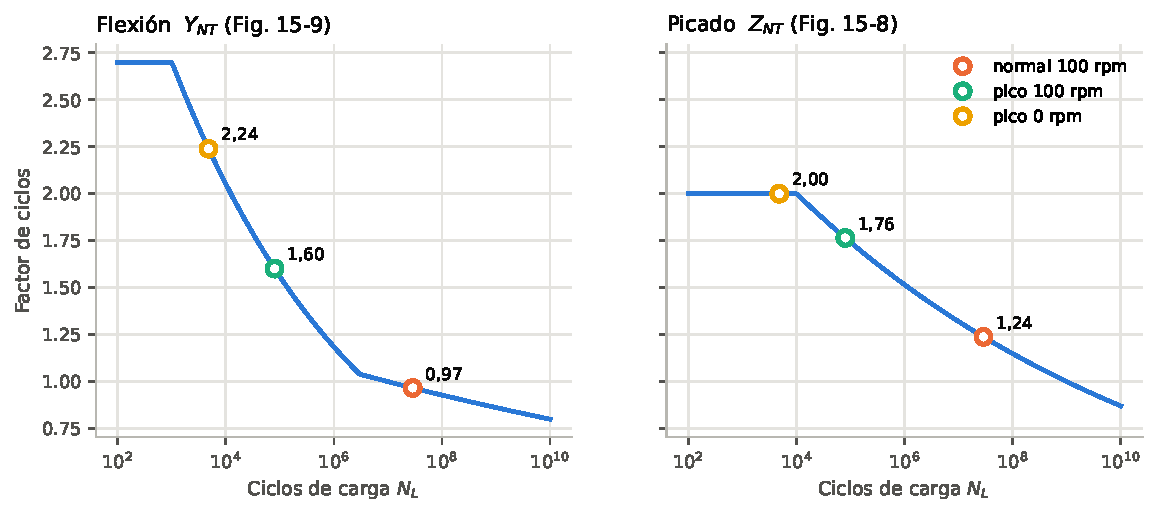
\includegraphics[width=0.95\linewidth]{figuras/fig_ciclos.pdf}\caption{Factores de ciclos de Shigley (Figs. 15-8 y 15-9, graficados desde sus ecuaciones) y puntos de trabajo. \textit{Fuente: ecuaciones de Shigley, cap. 15.}}\end{figure}


\section{Resistencia de los materiales}
El S45C sin tratamiento entra en Shigley como acero templado total grado~1. Se toma 170~HB, el extremo inferior de JIS G4051:
\begin{equation}
\sigma_{F\,\lim}=0{,}30\,\mathrm{HB}+14{,}48=65{,}5\ \text{MPa},\qquad
\sigma_{H\,\lim}=2{,}35\,\mathrm{HB}+162{,}89=562{,}4\ \text{MPa}
\end{equation}
El SUS304L (MIM) y el latón no figuran en Shigley. Se escalan desde el S45C con el mejor indicador disponible.
A flexión: la relación de resistencia de KG para el MIM (0,4) y la relación de límites de fatiga para el latón
(138/285). A picado: la dureza Brinell. El módulo elástico de cada par entra en $Z_E$:
\begin{equation}
Z_E=\left[\pi\left(\frac{1-\nu_1^2}{E_1}+\frac{1-\nu_2^2}{E_2}\right)\right]^{-1/2}
\end{equation}
\begin{table}[H]\centering\small\setlength{\tabcolsep}{4pt}
\caption{Propiedades y resistencias de referencia de los metales.}\label{tab:mat}
\begin{tabular}{l r r r r r p{3.2cm} r p{2.6cm}}
\toprule
Material & $E$ & $\nu$ & HB & $Z_E$ & $\sigma_{F\,\lim}$ & Base & $\sigma_{H\,\lim}$ & Base\\
 & GPa & & & $\sqrt{\text{MPa}}$ & MPa & & MPa & \\
\midrule
S45C & 205 & 0,30 & 170 & 189,4 & 65,5 & Shigley Fig. 15-13, grado 1, 170 HB & 562 & Shigley Fig. 15-12, grado 1, 170 HB \\
SUS304L (MIM) & 190 & 0,29 & 120 & 181,7 & 26,2 & KG: MIM = 0,4 $\times$ S45C & 397 & dureza 120/170 $\times$ S45C \\
Latón C3604B & 100 & 0,34 & 100 & 134,1 & 31,7 & fatiga 138/285 MPa $\times$ S45C & 331 & dureza 100/170 $\times$ S45C \\
\bottomrule\end{tabular}\end{table}


\section{Cálculo paso a paso: S45C, servicio normal a 100 rpm}
\begin{align*}
N_L &= 2\times(100\cdot60\cdot20\cdot12\cdot10) = 2{,}88\times10^{7}\\
v_{et} &= \pi\,d_e\,n/60\,000 = 0{,}0524\ \text{m/s} \;\Rightarrow\; K_v=1{,}0445\\
K_{H\beta} &= 1{,}25+5{,}6\times10^{-6}\,(2{,}121)^2=1{,}2500\\
Y_{NT} &= 1{,}6831\,N_L^{-0{,}0323}=0{,}9664,\qquad Z_{NT}=3{,}4822\,N_L^{-0{,}0602}=1{,}2382\\
\sigma_{FP} &= \frac{0{,}70\times65{,}48\times0{,}9664}{1\times1\times0{,}8952}=49{,}49\ \text{MPa}\\
\sigma_{HP} &= \frac{562{,}4\times1{,}2382}{1\times1\times0{,}9461}=736{,}0\ \text{MPa}\\
W_F &= \frac{49{,}49\times2{,}121\times0{,}5\times0{,}20}{1\times1{,}0445\times0{,}5\times1{,}2500}=16{,}08\ \text{N}
&&\Rightarrow\; T_F=0{,}0804\ \text{N\,m}\\
W_H &= \left(\frac{736{,}0}{189{,}4}\right)^2\frac{2{,}121\times10\times0{,}062}{1\times1{,}0445\times1{,}2500\times0{,}5\times2{,}0}=15{,}22\ \text{N}
&&\Rightarrow\; T_H=0{,}0761\ \text{N\,m}\\
T_{adm} &= \min(0{,}0804;\,0{,}0761)=\mathbf{0{,}0761\ \textbf{N\,m}}\quad\text{(picado)}
\end{align*}
Para los picos de 10~s a 100~rpm: $N_L=2\times2400\times16{,}7=8{,}00\times10^{4}$, $Y_{NT}=1{,}601$,
$Z_{NT}=1{,}765$ y $T_{adm}=0{,}1332$~N\,m (flexión).

\section{Resultados de los metales}
\begin{table}[H]\centering\scriptsize\setlength{\tabcolsep}{3.2pt}\caption{Servicio normal: ciclos de toda la vida (evaluados al doble, regla de Miner).}\begin{tabular}{l r r c c c r r r r r r r}
\toprule
Material & rpm & $N_L$ & $K_v$ & $Y_{NT}$ & $Z_{NT}$ & $\sigma_{FP}$ & $\sigma_{HP}$ & $W_F$ & $W_H$ & $T_F$ & $T_H$ & $T_{adm}$\\
 & & & & & & MPa & MPa & N & N & N\,m & N\,m & N\,m\\
\midrule
S45C & 0,5 & $1{,}44\times10^{5}$ & 1,0032 & 1,493 & 1,703 & 76,5 & 1013 & 25,9 & 30,0 & 0,129 & 0,150 & \textbf{0,129} \\
S45C & 50 & $1{,}44\times10^{7}$ & 1,0315 & 0,988 & 1,291 & 50,6 & 767 & 16,7 & 16,8 & 0,083 & 0,084 & \textbf{0,083} \\
S45C & 100 & $2{,}88\times10^{7}$ & 1,0445 & 0,966 & 1,238 & 49,5 & 736 & 16,1 & 15,2 & 0,080 & 0,076 & \textbf{0,076} \\
SUS304L (MIM) & 0,5 & $1{,}44\times10^{5}$ & 1,0032 & 1,493 & 1,703 & 30,6 & 715 & 10,3 & 16,2 & 0,052 & 0,081 & \textbf{0,052} \\
SUS304L (MIM) & 50 & $1{,}44\times10^{7}$ & 1,0315 & 0,988 & 1,291 & 20,2 & 542 & 6,7 & 9,1 & 0,033 & 0,045 & \textbf{0,033} \\
SUS304L (MIM) & 100 & $2{,}88\times10^{7}$ & 1,0445 & 0,966 & 1,238 & 19,8 & 520 & 6,4 & 8,2 & 0,032 & 0,041 & \textbf{0,032} \\
Latón C3604B & 0,5 & $1{,}44\times10^{5}$ & 1,0032 & 1,493 & 1,703 & 37,0 & 596 & 12,5 & 20,7 & 0,063 & 0,103 & \textbf{0,063} \\
Latón C3604B & 50 & $1{,}44\times10^{7}$ & 1,0315 & 0,988 & 1,291 & 24,5 & 451 & 8,1 & 11,5 & 0,040 & 0,058 & \textbf{0,040} \\
Latón C3604B & 100 & $2{,}88\times10^{7}$ & 1,0445 & 0,966 & 1,238 & 24,0 & 433 & 7,8 & 10,5 & 0,039 & 0,052 & \textbf{0,039} \\
\bottomrule\end{tabular}\end{table}

\begin{table}[H]\centering\scriptsize\setlength{\tabcolsep}{3.2pt}\caption{Picos de 10 s: ciclos de los picos (evaluados al doble, regla de Miner).}\begin{tabular}{l r r c c c r r r r r r r}
\toprule
Material & rpm & $N_L$ & $K_v$ & $Y_{NT}$ & $Z_{NT}$ & $\sigma_{FP}$ & $\sigma_{HP}$ & $W_F$ & $W_H$ & $T_F$ & $T_H$ & $T_{adm}$\\
 & & & & & & MPa & MPa & N & N & N\,m & N\,m & N\,m\\
\midrule
S45C & 0 & $4{,}80\times10^{3}$ & 1,0000 & 2,240 & 2,000 & 114,7 & 1189 & 38,9 & 41,5 & 0,195 & 0,207 & \textbf{0,195} \\
S45C & 0,5 & $4{,}80\times10^{3}$ & 1,0032 & 2,240 & 2,000 & 114,7 & 1189 & 38,8 & 41,3 & 0,194 & 0,207 & \textbf{0,194} \\
S45C & 50 & $4{,}00\times10^{4}$ & 1,0315 & 1,739 & 1,840 & 89,1 & 1094 & 29,3 & 34,0 & 0,147 & 0,170 & \textbf{0,147} \\
S45C & 100 & $8{,}00\times10^{4}$ & 1,0445 & 1,601 & 1,765 & 82,0 & 1049 & 26,6 & 30,9 & 0,133 & 0,155 & \textbf{0,133} \\
SUS304L (MIM) & 0 & $4{,}80\times10^{3}$ & 1,0000 & 2,240 & 2,000 & 45,9 & 839 & 15,6 & 22,4 & 0,078 & 0,112 & \textbf{0,078} \\
SUS304L (MIM) & 0,5 & $4{,}80\times10^{3}$ & 1,0032 & 2,240 & 2,000 & 45,9 & 839 & 15,5 & 22,4 & 0,078 & 0,112 & \textbf{0,078} \\
SUS304L (MIM) & 50 & $4{,}00\times10^{4}$ & 1,0315 & 1,739 & 1,840 & 35,6 & 772 & 11,7 & 18,4 & 0,059 & 0,092 & \textbf{0,059} \\
SUS304L (MIM) & 100 & $8{,}00\times10^{4}$ & 1,0445 & 1,601 & 1,765 & 32,8 & 740 & 10,7 & 16,7 & 0,053 & 0,084 & \textbf{0,053} \\
Latón C3604B & 0 & $4{,}80\times10^{3}$ & 1,0000 & 2,240 & 2,000 & 55,5 & 699 & 18,8 & 28,6 & 0,094 & 0,143 & \textbf{0,094} \\
Latón C3604B & 0,5 & $4{,}80\times10^{3}$ & 1,0032 & 2,240 & 2,000 & 55,5 & 699 & 18,8 & 28,5 & 0,094 & 0,143 & \textbf{0,094} \\
Latón C3604B & 50 & $4{,}00\times10^{4}$ & 1,0315 & 1,739 & 1,840 & 43,1 & 643 & 14,2 & 23,5 & 0,071 & 0,117 & \textbf{0,071} \\
Latón C3604B & 100 & $8{,}00\times10^{4}$ & 1,0445 & 1,601 & 1,765 & 39,7 & 617 & 12,9 & 21,3 & 0,065 & 0,107 & \textbf{0,065} \\
\bottomrule\end{tabular}\end{table}

\begin{figure}[H]\centering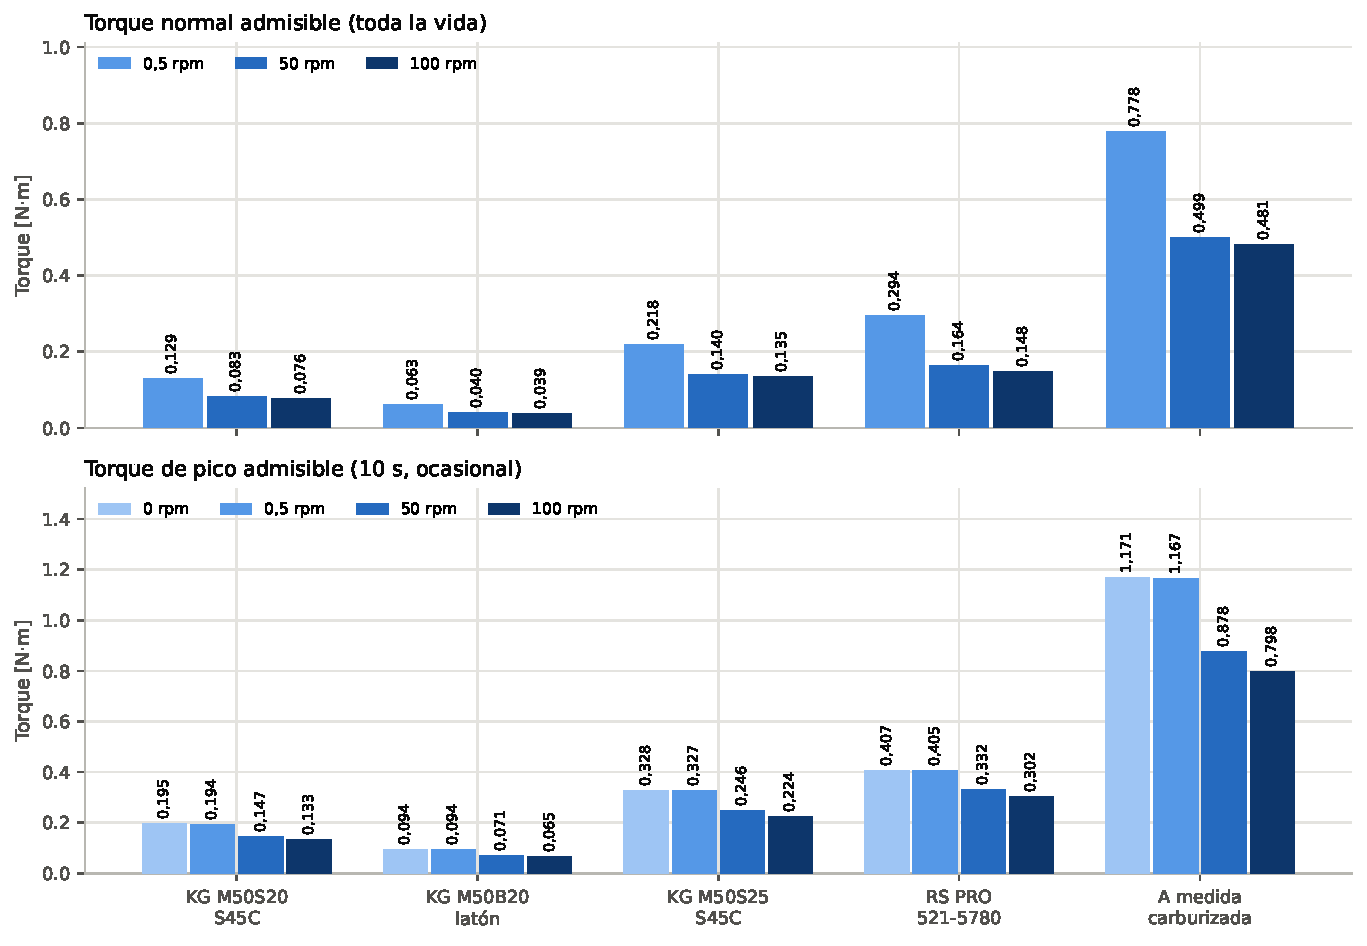
\includegraphics[width=\linewidth]{figuras/fig_resumen.pdf}\caption{Torque admisible por material y velocidad: servicio normal y picos. \textit{Fuente: cálculo propio.}}\label{fig:resumen}\end{figure}

\begin{figure}[H]\centering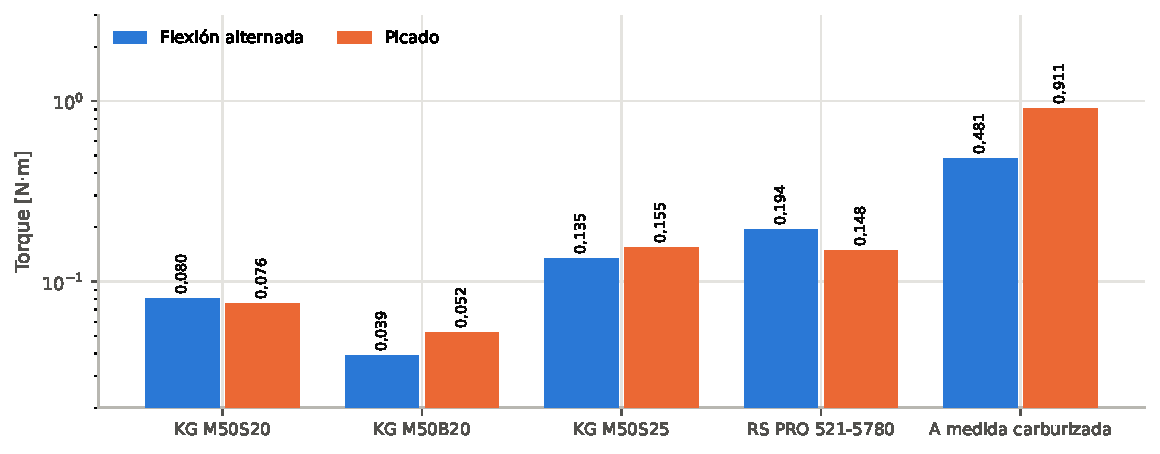
\includegraphics[width=\linewidth]{figuras/fig_modos.pdf}\caption{Servicio normal a 100 rpm: flexión alternada y picado según Shigley frente a la tabla de KG. \textit{Fuente: cálculo propio; KG, catálogo KG4001.}}\end{figure}

\begin{figure}[H]\centering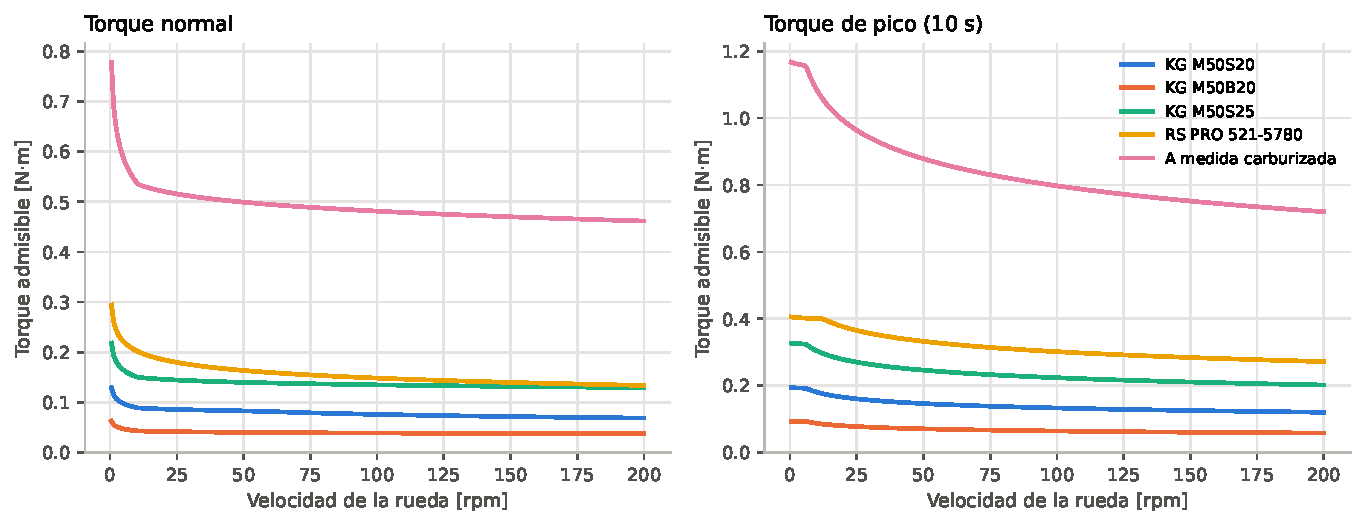
\includegraphics[width=\linewidth]{figuras/fig_rpm.pdf}\caption{Torque admisible en función de la velocidad de la rueda. \textit{Fuente: cálculo propio.}}\end{figure}

Todos los picos cumplen además $\sigma_{FP}<S_y$: no hay fluencia estática del diente.

\section{POM inyectado}\label{sec:pom}
Las ecuaciones AGMA valen solo para metales. Para plásticos, KG y KHK usan la ecuación de Lewis con factores de servicio:
\begin{equation}
T=\frac{d_e}{2}\;m\,y\,b\,\sigma_{b\,\mathrm{adm}}\,\frac{R_e-b}{R_e},\qquad
\sigma_{b\,\mathrm{adm}}=0{,}70\;\sigma_b(N)\,\frac{K_V\,K_T\,K_L\,K_M}{C_S}
\end{equation}
con $\sigma_b(N)$ de la curva m\,0,8 de KHK, $K_V=1{,}4$ ($v\approx0$; 1 en estático), $K_T=0{,}80$ (40\,$^\circ$C),
$K_L=1$ (grasa), $K_M=0{,}75$ (POM contra POM), $C_S=1{,}25$ en servicio normal y $0{,}80$ en picos.
Se adopta la menor de tres estimaciones: el método KHK, Lewis con el factor $Y$ de Shigley (tabla 14-2)
y la tabla de KG del POM azul m\,0,8 escalada a m\,0,5.
\begin{table}[H]\centering\small\setlength{\tabcolsep}{4pt}
\caption{POM inyectado: tres estimaciones y valor adoptado (N\,m), carga alternada incluida.}\label{tab:pom}
\begin{tabular}{l r r r r r r r r r}
\toprule
Régimen & rpm & $N$ & $\sigma_b(N)$ & $C_S$ & $\sigma_{b\,\mathrm{adm}}$ & KHK & Lewis--Shigley & Calibrado KG & Adoptado\\
 & & & MPa & & MPa & $y=0{,}597$ & $Y=0{,}353$ & & \\
\midrule
Normal & 0,5 & $1{,}44\times10^{5}$ & 48,6 & 1,25 & 22,9 & 0,055 & 0,033 & 0,025 & \textbf{0,025} \\
Normal & 50 & $1{,}44\times10^{7}$ & 38,7 & 1,25 & 18,2 & 0,044 & 0,026 & 0,020 & \textbf{0,020} \\
Normal & 100 & $2{,}88\times10^{7}$ & 37,6 & 1,25 & 17,7 & 0,043 & 0,025 & 0,020 & \textbf{0,020} \\
Pico & 0 & $4{,}80\times10^{3}$ & 55,4 & 0,80 & 29,1 & 0,070 & 0,041 & 0,021 & \textbf{0,021} \\
Pico & 0,5 & $4{,}80\times10^{3}$ & 55,4 & 0,80 & 40,7 & 0,098 & 0,058 & 0,029 & \textbf{0,029} \\
Pico & 50 & $4{,}00\times10^{4}$ & 52,5 & 0,80 & 38,6 & 0,093 & 0,055 & 0,027 & \textbf{0,027} \\
Pico & 100 & $8{,}00\times10^{4}$ & 50,2 & 0,80 & 36,9 & 0,089 & 0,053 & 0,026 & \textbf{0,026} \\
\bottomrule\end{tabular}\end{table}

\begin{minipage}{0.49\linewidth}\centering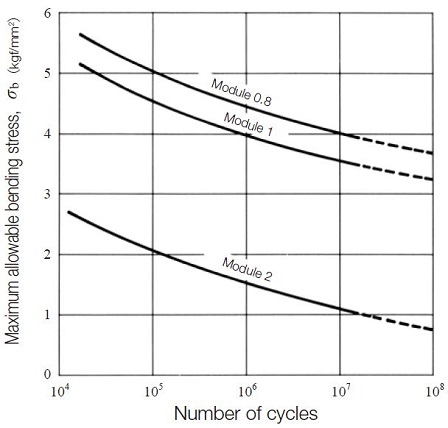
\includegraphics[width=0.95\linewidth]{capturas/Fig.11.3.jpg}
\captionof{figure}{Esfuerzo admisible de flexión del POM (Duracon). \textit{Fuente: KHK, Fig. 11.3.}}\end{minipage}\hfill
\begin{minipage}{0.49\linewidth}\centering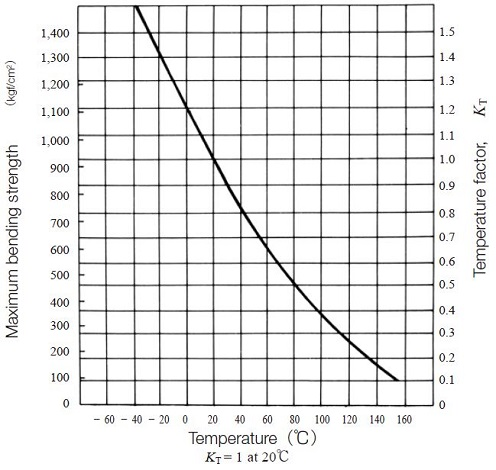
\includegraphics[width=0.95\linewidth]{capturas/Fig.-11.5-Temperature-factor-KT.jpg}
\captionof{figure}{Factor de temperatura $K_T$. \textit{Fuente: KHK, Fig. 11.5.}}\end{minipage}

\begin{caja}[orange!80!black]{Advertencias del POM}
El POM absorbe humedad, se dilata con la temperatura y fluye (creep) bajo torque sostenido a 40\,$^\circ$C.
El valor a 0~rpm vale para picos de 10~s, no para retener la rueda durante minutos.
\end{caja}

\section{Sensibilidad}
\begin{figure}[H]\centering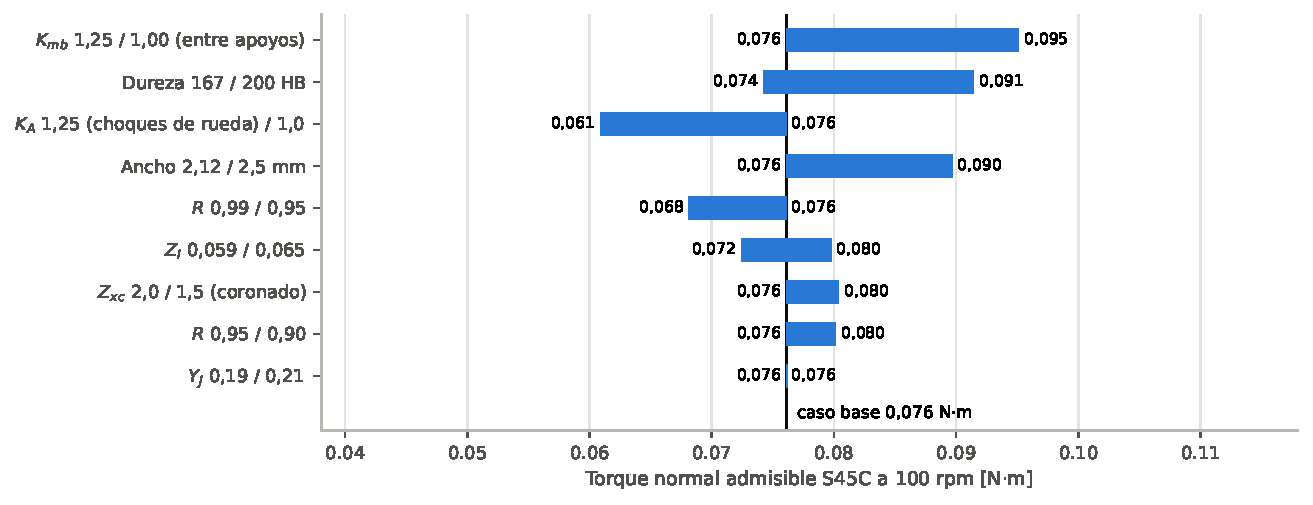
\includegraphics[width=\linewidth]{figuras/fig_sensibilidad.pdf}\caption{Sensibilidad del torque normal del S45C a 100 rpm a cada supuesto. \textit{Fuente: cálculo propio.}}\label{fig:sens}\end{figure}

\begin{figure}[H]\centering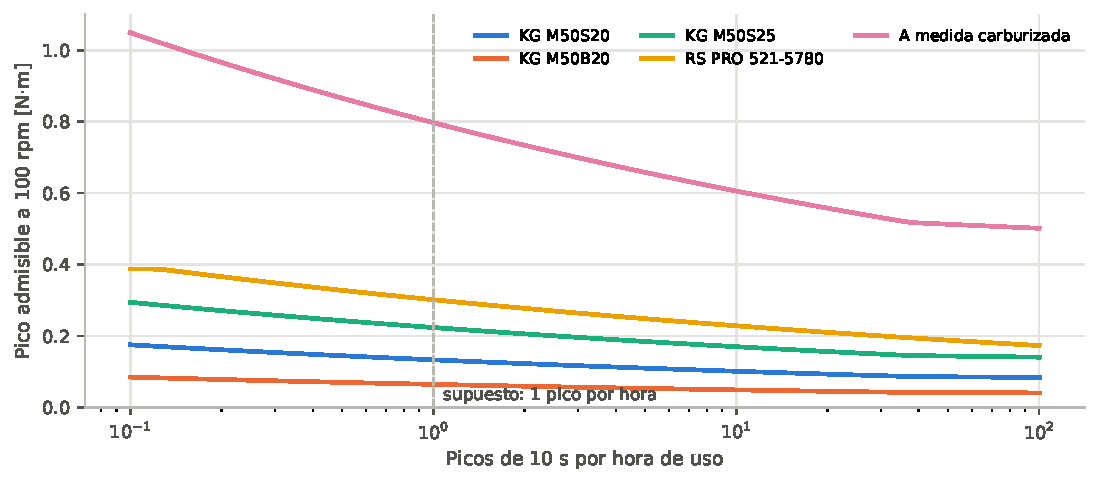
\includegraphics[width=\linewidth]{figuras/fig_picos.pdf}\caption{Torque de pico admisible a 100 rpm en función de la frecuencia de picos. \textit{Fuente: cálculo propio.}}\end{figure}

\begin{table}[H]\centering\small
\caption{Torque normal con hipótesis pesimistas de picado para materiales no tabulados por Shigley (N\,m).}
\begin{tabular}{l l rr rr}
\toprule
 & Hipótesis alternativa & \multicolumn{2}{c}{50 rpm} & \multicolumn{2}{c}{100 rpm}\\
\cmidrule(lr){3-4}\cmidrule(lr){5-6}
Material & & adoptado & cota baja & adoptado & cota baja\\
\midrule
SUS304L (MIM) & $\sigma_{H\,\lim}=0{,}40\times$ S45C & 0,033 & 0,015 & 0,032 & 0,013 \\
Latón C3604B & $\sigma_{H\,\lim}=0{,}36\times$ S45C (bronce, Shigley tabla 14-7) & 0,040 & 0,021 & 0,039 & 0,019 \\
\bottomrule\end{tabular}\end{table}


\section{Alternativas para aumentar el torque con $d_a\le14$ mm}\label{sec:alt}
El torque de un cónico crece con el diámetro, el módulo, el ancho útil ($\le0{,}3R_e$) y la resistencia superficial del material.
Con el diámetro exterior limitado a 14~mm, las opciones son:
\begin{itemize}
\item \textbf{B -- KG M50S25 (stock).} m\,0,5, 25 dientes, $d_a=13{,}21$ mm, $b=3$ mm. Es el mismo proveedor y el mismo tipo de montaje
(agujero $\varnothing4$). $J=0{,}216$ e $I=0{,}065$ se tomaron del Ejemplo 15-1 de Shigley (mitras de 25 dientes).
\item \textbf{C -- KG M50B25 (latón, stock).} Mismo tamaño en latón. No mejora frente al S45C de 20 dientes.
\item \textbf{D -- RS PRO 521-5780 (acero, stock).} m\,0,8, 16 dientes, $d_a\approx13{,}9$ mm. El ancho de cara ($0{,}3R_e$ supuesto), $J$ e $I$
(extrapolados a 16 dientes) deben confirmarse con la hoja de datos.
\item \textbf{E -- A medida, m\,0,6 $\times$ 21, S45C.} Módulo normalizado, $d_a=13{,}45$ mm.
\item \textbf{F/G -- A medida, carburizado (SCM415, 58--62 HRC).} Shigley, acero carburizado grado~1:
$\sigma_{F\,\lim}=206{,}8$ MPa y $\sigma_{H\,\lim}=1379$ MPa. Es la mejora más grande, a costa de fabricación especial.
\end{itemize}
\begin{table}[H]\centering\scriptsize\setlength{\tabcolsep}{3pt}
\caption{Alternativas con diámetro exterior $d_a\le 14$ mm (relación 1:1, 90$^\circ$). Torques en N\,m por engranaje.}\label{tab:alt}
\begin{tabular}{c p{3.3cm} l r r r r r r r r}
\toprule
 & Producto & Material & $m$ & $z$ & $d_a$ & $b_{ef}$ & Normal & Pico & Pico & Relación\\
 & & & mm & & mm & mm & 100 rpm & 100 rpm & 0 rpm & vs.\ A\\
\midrule
A & Referencia: KG M50S20 & S45C & 0,50 & 20 & 10,71 & 2,12 & 0,076 & 0,133 & 0,195 & 1,0 \\
B & KG M50S25 (stock) & S45C & 0,50 & 25 & 13,21 & 2,65 & 0,135 & 0,224 & 0,328 & 1,8 \\
C & KG M50B25 (stock) & Latón C3604B & 0,50 & 25 & 13,21 & 2,65 & 0,065 & 0,108 & 0,159 & 0,9 \\
D & RS PRO 521-5780 (stock) & S45C & 0,80 & 16 & 13,93 & 2,72 & 0,148 & 0,302 & 0,407 & 2,0 \\
E & A medida, S45C & S45C & 0,60 & 21 & 13,45 & 2,67 & 0,151 & 0,253 & 0,371 & 2,0 \\
F & A medida, m0,5 carburizado & SCM415 carburizado & 0,50 & 20 & 10,71 & 2,12 & 0,254 & 0,421 & 0,615 & 3,3 \\
G & A medida, m0,6 carburizado & SCM415 carburizado & 0,60 & 21 & 13,45 & 2,67 & 0,481 & 0,798 & 1,171 & 6,3 \\
\bottomrule\end{tabular}\end{table}

\begin{figure}[H]\centering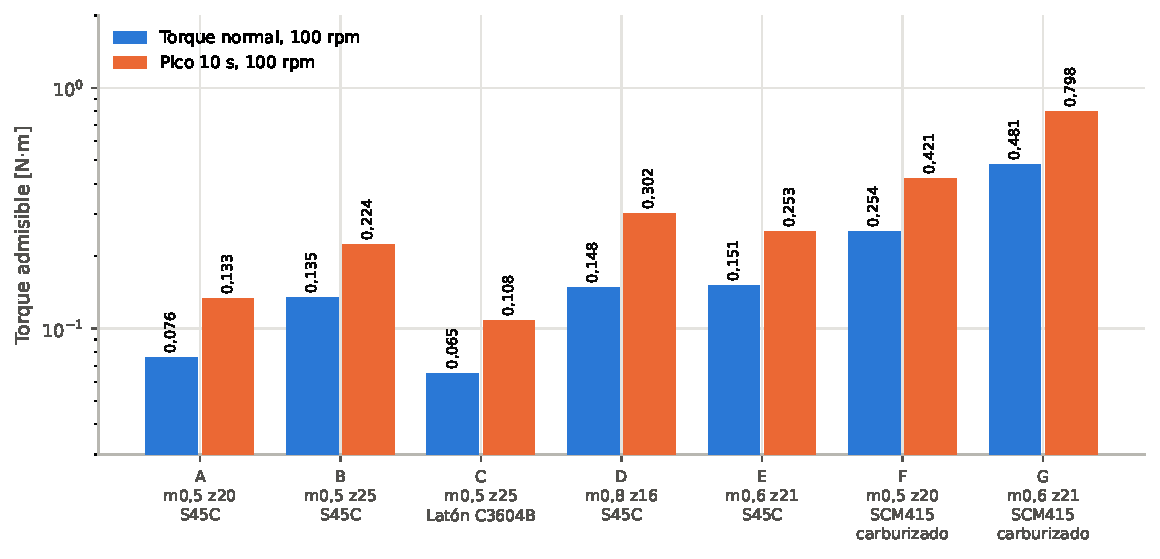
\includegraphics[width=\linewidth]{figuras/fig_alternativas.pdf}\caption{Torque admisible de las alternativas a 100 rpm (escala logarítmica). \textit{Fuente: cálculo propio.}}\end{figure}

\begin{caja}{Recomendación}
Como cambio inmediato con piezas de stock y el mismo proveedor: \textbf{KG M50S25} (B), con $\times$1,8
en servicio normal y 0,328~N\,m de pico a rueda detenida.
Si hace falta más, una mitra a medida \textbf{m\,0,6 $\times$ 21 carburizada} (G). Con esa capacidad la fijación y el eje pasan a ser el límite
(sección~\ref{sec:verif}): prever chaveta o plano de arrastre y un eje de $\varnothing4$ o mayor.
\end{caja}

\section{Lubricación}\label{sec:lub}
\textbf{Sí, es imprescindible.}
\begin{enumerate}[leftmargin=1.2em]
\item \textbf{El método la supone.} Las capacidades AGMA de Shigley y las tablas de KG (baño de aceite de 100~cSt)
valen para engranajes lubricados. En seco los valores de este informe no son válidos: domina el desgaste adhesivo.
\item \textbf{Régimen de lubricación límite.} A $v_{et}\approx0{,}03$--$0{,}05$ m/s no se forma película elastohidrodinámica.
Los flancos se separan solo por la capa adsorbida de la grasa, así que el modo de falla a largo plazo es el
\textbf{desgaste}, que AGMA no calcula. Se necesita grasa con aditivos de extrema presión (EP) y antidesgaste, o con lubricante sólido (MoS$_2$).
\item \textbf{Materiales.} El S45C sin tratamiento se oxida (una rueda puede recibir humedad). El SUS304L contra SUS304L tiende a gripar
(\textit{galling}), así que en seco fallaría rápido. El latón tolera mejor la marcha pobre de lubricante, pero se desgasta. El POM puede andar en seco,
pero la grasa reduce el desgaste y el calentamiento.
\item \textbf{Recomendación práctica.} Grasa semifluida NLGI 00--0 (penetra y vuelve al engrane) de complejo de litio con EP para los metales.
Para POM, grasa sintética compatible con plásticos. Compartimiento cerrado contra polvo y arena, que en una rueda actúan como abrasivo.
Reengrase en cada mantenimiento y control del juego tras las primeras campañas.
\end{enumerate}

\section{Verificaciones adicionales}\label{sec:verif}
\begin{itemize}
\item \textbf{Prisioneros.} Shigley tabla 7-4: un prisionero n.º~2 sujeta 85~lbf $\approx378$~N. Sobre $\varnothing3$ mm son
0,57~N\,m por tornillo, 0,28~N\,m con factor 2. Alcanza para los picos del S45C
(0,195~N\,m), siempre que el eje tenga un plano de apoyo. \textbf{No alcanza para las alternativas D a G.}
\item \textbf{Eje $\varnothing3$ mm.} Con el mayor pico (0,195~N\,m): $\tau=16T/(\pi d^3)=36,7$ MPa, admisible para acero.
\item \textbf{Golpes de la rueda.} Si la rueda choca contra obstáculos o el carro frena bruscamente, $K_A=1{,}25$ y todos los valores bajan un 20\,\%.
\end{itemize}

\section{Conclusiones}
\begin{enumerate}[leftmargin=1.2em]
\item Con Shigley ($R=0{,}95$, carga alternada, 10 años), la mitra KG m\,0,5 $\times$ 20 en S45C admite
0,083 y 0,076~N\,m de torque normal a 50 y 100~rpm, y picos de 10~s de
0,147 y 0,133~N\,m (0,195~N\,m a rueda detenida).
\item El latón admite alrededor de la mitad, el MIM un 40\,\% y el POM un 25\,\% de esos valores.
\item El dato de KG no representa la capacidad del par en esta aplicación.
\item Dentro de 14~mm, el reemplazo directo es KG M50S25. Con fabricación a medida carburizada se llega a más de seis veces la capacidad actual.
\item La lubricación con grasa EP es condición necesaria de todos los valores de este informe.
\end{enumerate}

\section*{Referencias}
\addcontentsline{toc}{section}{Referencias}
\begin{enumerate}[label={[\arabic*]},leftmargin=2em]
\item Budynas, R.\,G. y Nisbett, J.\,K. \textit{Diseño en ingeniería mecánica de Shigley}, 10.ª ed. McGraw-Hill. Caps. 6, 7 (tabla 7-4), 14 (tablas 14-2 y 14-7) y 15.
\item KG (Kyoiku Gear Mfg.). Catálogo KG4001, sección de mitras, pp. 233--276. \url{https://www.kggear.co.jp/wp-content/uploads/2022/11/KG4001WEB-7.pdf}
\item KG. Catálogo KG3001, pp. 379--444. \url{https://www.kggear.co.jp/wp-content/uploads/KG3001_web_0009.pdf}
\item KG. Material de referencia KG5001, pp. 18 y 20. \url{https://www.kggear.co.jp/wp-content/uploads/2024/06/KG5001JP_reference.pdf}
\item KG. \textit{Technical Data Note}, cap. 10.2. \url{https://www.kggear.co.jp/en/wp-content/themes/bizvektor-global-edition/pdf/TechnicalData_KGSTOCKGEARS.pdf}
\item KHK. \textit{Design of Plastic Gears}. \url{https://khkgears.net/new/gear_knowledge/gear_technical_reference/design-of-plastic-gears.html}
\item KHK. \textit{Hardened Miter Gears (SMA/SMB/SMC)}. \url{https://www.khkgears.us/catalog/category/hardened_miter_gears_sma-smb-smc/}
\item RS Components. RS PRO Steel Mitre Gear, 0,8 Module, 16 Teeth, 521-5780. \url{https://ie.rs-online.com/web/p/mitre-bevel-gears/5215780}
\item Copper Development Association. C36000 Free-Cutting Brass. \url{https://www.copper.org/applications/rodbar/alloy360/free_cutting.html}
\end{enumerate}
\end{document}
